\begin{figure}[h!]
  \centering    
    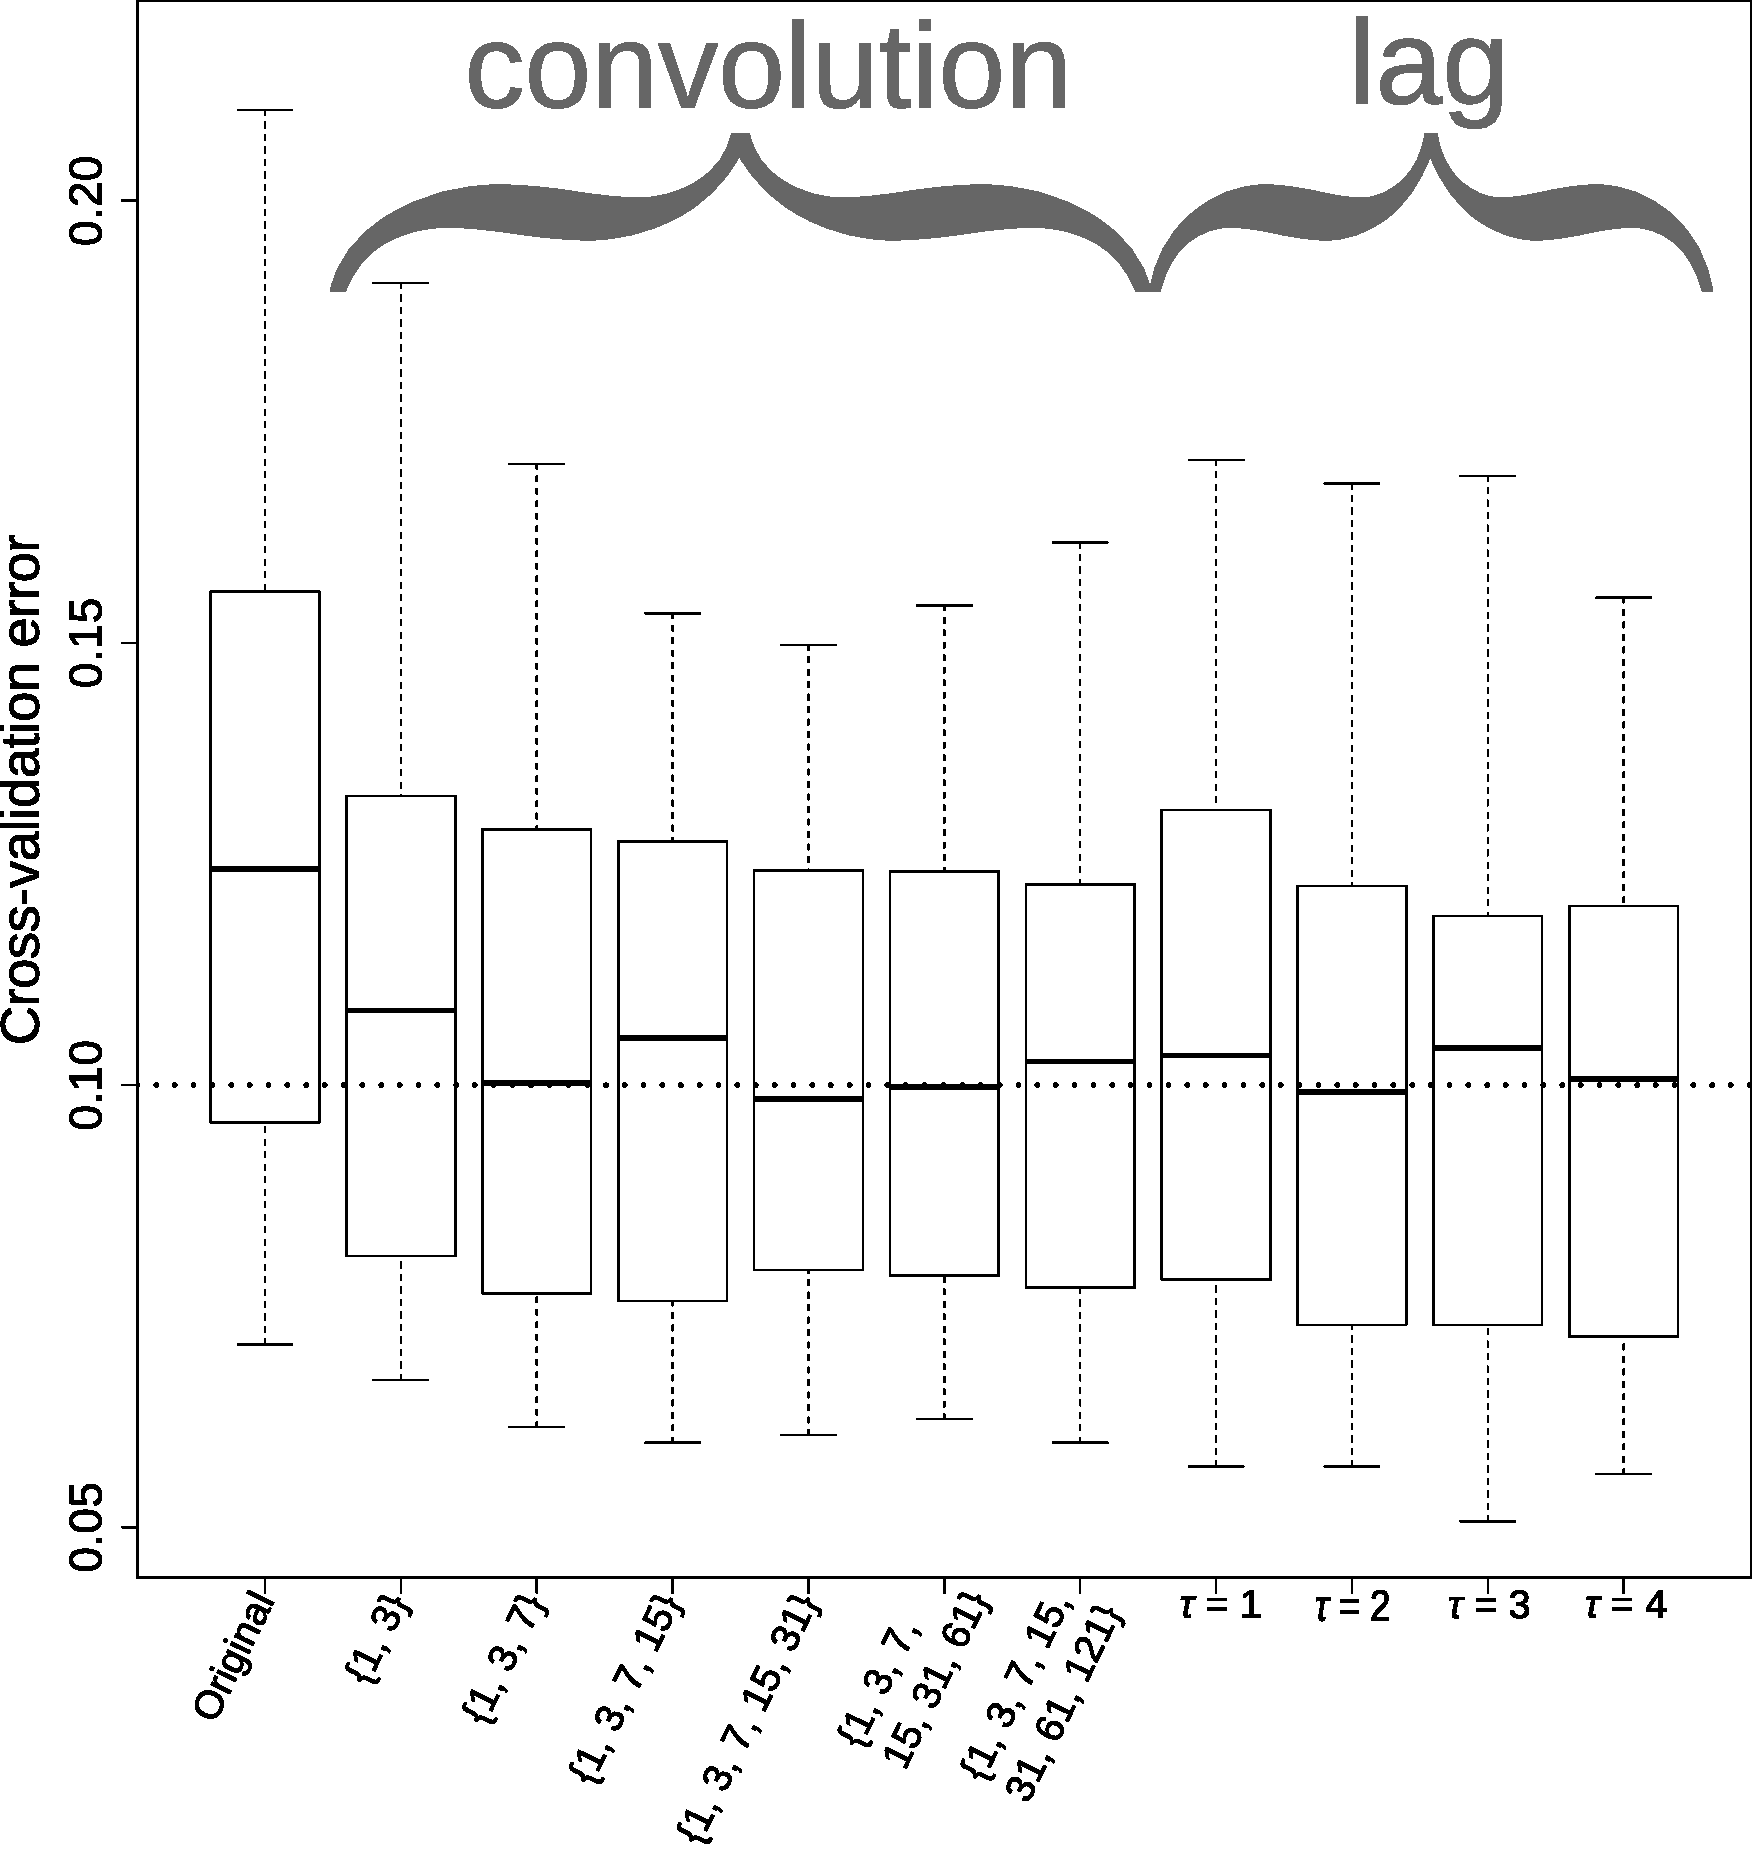
\includegraphics[width=0.5\textwidth]{figures/temporal_integration.pdf}
  \caption{\ctit{Integration of temporal information.}
  In order to improve prediction accuracy, information about the past and future features was added to the original features following two different strategies.
  Convolution inflates $p$ by adding the mean features of neighbouring points over different window sizes (eq.~\ref{eq:window}).
  The numbers in braces represent the window sizes.
  Alternatively, the features of the $\tau$ previous and future neighbours was added to the variables (eq.~\ref{eq:tau}).
  The dotted line represents a cross-validation error of $10\%$.
  All additions of temporal features reduce significantly the cross-validation error compared to the original set of features ($p-value < 5.10^{-3}$, for all, repeated t-tests).
  Significance threshold, $\alpha = 0.05$, after Bonferroni correction is $\alpha' = 0.05/10 = 5.10^{-3}$.
  \label{fig:temporal_integration}
  }
\end{figure}
